\section{Results}

\subsection{Hypotheses}

We wish to test the following hypotheses.

\newtheorem{policyWorks}{Hypothesis}

\begin{policyWorks}
	The number of comments a user receives from community managers has no influence on her probability to be active.
	\label{hypothesis:policyWorks}
\end{policyWorks}

The organisations running online communities wish for their users to do certain things, most of which imply being active in the community itself: writing posts and comments. They cannot order them to do so, since users are not on the payroll and remain unanswerable to those organisations. Online community managers are then tasked to prompt users into action without using either monetary incentives or command power. That leaves interaction as the main tool online community managers have at their disposal. Rejecting Hypothesis \ref{hypothesis:policyWorks} would imply that users do, in fact, respond to cues from online community managers.

We expect Hypothesis \ref{hypothesis:policyWorks} to be falsified by data. Moreover, we expect that the coefficient on the number of comments received by the user from community managers, besides being statistically different from zero, is positive. Denote said coefficient by  $\beta_{cmrec}$, and the related variable by $x_{cmrec}$. Check that: 

\begin{equation}
	\frac{\partial Pr(A=1|x)}{\partial x_{cmrec}} > 0 \Rightarrow \frac{\partial LOR}{\partial x_{cmrec}} > 0
	\label{marginalProbActive}
\end{equation}

where $LOR$ denotes the logarithm of the log-odds ratio as per equation \ref{eq:logOddsErrors}. Since $x_{cmrec}$ enters equation \ref{eq:logOdds} linearly, equation \ref{marginalProbActive} implies that:

\begin{equation}
	\frac{\partial LOR}{\partial x_{cmrec}} > 0 \Rightarrow \beta_{cmrec} > 0 
\end {equation}

\begin{policyWorks}
	Receiving comments from community managers has the same effect on the probability to be active than receiving comments from users that are not community managers. 
	\label{hypothesis:policyWorksBetter}
\end{policyWorks}

Online community managers are professionals. They are likely to have better communication skills than the average user, and they certainly have stronger incentives to craft their interaction modes so as to drive users to being more active in the online community. We therefore expect, on average, the effect of incoming communication from online community manager to have a larger positive effect on the probability of becoming active than that of incoming communication from other users. Therefore, we expect Hypothesis \ref{hypothesis:policyWorksBetter} to be falsified by the data. 

\begin{policyWorks}
	Receiving an additional comment from a community manager has a large effect on the probability that a user becomes active. 	
	\label{hypothesis:policyWorksWell}
\end{policyWorks}

The number of comments authored by online community manager is the main policy variable in Edgeryders and other online communities like it. Employing community managers would not make economic sense if their impact on the level of activity in the community was not large enough. Hypothesis \ref{hypothesis:policyWorksWell} is more restrictive than Hypothesis \ref{hypothesis:policyWorks}, as it implies that the policy variable, the number of comments received from community manager, has a marginal effect that is not only statistically distinguishable from zero, but also sizeable. For example, if targeting users with a comment only increased their probability of being active by a few percent, many businesses running online communities would probably reconsider their decision to hire a community manager. 

\subsection{Regression}

Table \ref{tab:xtlogit} summarizes the estimation's results. 


\def\onepc{$^{\ast\ast}$} \def\fivepc{$^{\ast}$}
\def\tenpc{$^{\dag}$}
\def\legend{\multicolumn{4}{l}{\footnotesize{Significance levels
:\hspace{1em} $\dag$ : 10\% \hspace{1em}
$\ast$ : 5\% \hspace{1em} $\ast\ast$ : 1\% \normalsize}}}
\begin{table}[htbp]\centering
\begin{tabular}{l r @{} l c }\hline\hline 
\multicolumn{1}{c}
{\textbf{Variable}}
 & \multicolumn{2}{c}{\textbf{Coefficient}}  & \textbf{(Std. Err.)} \\ \hline
n. comments received from community managers  &  1.250&\onepc  & (0.053)\\
n. comments received from other users  &  0.215&\onepc  & (0.037)\\
n. comments and posts written by ego (lagged)  &  0.126&\tenpc  & (0.066)\\
weeks since creating the account  &  -0.011&\tenpc  & (0.006)\\
n. of posts and comments written by users excluding ego  &  0.037&\onepc  & (0.004)\\
n. of posts and comments written by community managers  &  0.001&  & (0.006)\\
user out-degree (lagged) &  0.028&\fivepc  & (0.013)\\
user in-degree (lagged)  &  -0.003&  & (0.013)\\
user betweenness centrality  &  -107.870&\onepc  & (20.778)\\
user pagerank (lagged) &  -5.592&  & (14.610)\\
user clustering coefficient  &  -0.654&\onepc  & (0.195)\\
network average distance  &  -4.156&\fivepc  & (2.007)\\
network average betweenness centrality at $t-1$  &  -9.260&  & (209.212)\\
network Louvain modularity  &  8.379&\onepc  & (2.520)\\
n. nodes  &  -0.001&  & (0.004)\\
n. edges  &  0.000&  & (0.001)\\
\hline
\onepc = 1\% significant; \fivepc = 5\% significant; \tenpc = 10\% significant.

\end{tabular}
 \caption{Estimation results for the dependent variable $A_{i,t}$}
\label{tab:xtlogit}
\end{table}


The coefficients on the first two variables are positive and highly significant ($p < 0.001$). This supports the conventional wisdom that users of online communities tend to engage with each other: when made the object of comments, they are more likely to become active than when they are not. By implication, our Hypothesis \ref{hypothesis:policyWorks} must be rejected. 

To test Hypothesis \ref{hypothesis:policyWorksBetter}, we start by noting that the coefficient on the number of comments received from community managers is larger than that on the number of comments received from other (non-community managers) users. We next run a Wald test on the null hypothesis that the coefficients on our first two variables are identical. The null is strongly rejected ($p < 0.0001$). This, in turn, means we have no support for Hypothesis \ref{hypothesis:policyWorksBetter}. 

Ideally, we would like that to support the alternative hypothesis that the difference between the coefficient on the number of comments received by the user from community managers and the coefficient on the number of comments received by other (non-community managers) users be positive. Wald tests, being one-tailed, cannot do that. However, we can deduce the non-negativity of such difference from the signs and values of the estimated coefficients and our functional form in equation \ref{eq:logOddsErrors}. Formally, denote the  coefficient on the number of comments received by other (non-community managers) users by $\beta_{urec}$, and the related variable by $x_{urec}$. Since the transformation from probability to odds is monotonic, we have:

\begin{equation}
	\frac{\partial Pr(A=1|x)}{\partial x_{cmrec}} > \frac{\partial Pr(A=1|x)}{\partial x_{urec}}  \Rightarrow \frac{\partial LOR}{\partial x_{cmrec}} > \frac{\partial LOR}{\partial x_{urec}} 
\end{equation}

Applying again equation \ref{eq:logOddsErrors}, and remembering that both $x_{cmrec}$ and $x_{urec}$ enter it linearly, we have:

\begin{equation}
	\frac{\partial LOR}{\partial x_{cmrec}} > \frac{\partial LOR}{\partial x_{urec}}\Rightarrow \beta_{cmrec} > \beta_{urec} \Rightarrow \beta_{cmrec} - \beta_{urec} > 0
	\label{eq:condition4WaldTest}
\end{equation}

So, the difference $\beta_{cmrec} - \beta_{urec}$ cannot be negative. Since we have strongly rejected that it be zero, it follows that it must be strictly positive. The activation effect of receiving comments from online community managers is thus significantly greater than that of receiving comments from ordinary users.

\subsection{Marginal effects}

Regression analysis shows that the activity of community managers does indeed have a positive impact on the probability that the users they engage will become active. This, however, does not tell us how large that impact is. Since online community management is costly, this is likely to be a question of some relevance to an organisation trying to make a decision to invest in it. 
Coefficient estimates are a poor indicator of marginal effects, because the logit model we employ here is not linear. The relationship between the linear prediction (as defined by the sum of each coefficient multiplied by the regressor it refers to, and assuming the fixed effects are zero) and the probability that the dependent variable is equal to 1 follows a logistic curve (figure \ref{fig:probActivityLinPredict}). An increase in the number of comments received by community managers has a small effect for small or large values of $x\beta$. When $x\beta$ is between -5 and 5, however, the probability that the user becomes active increases quickly as community managers engage more with the user.

\begin{figure}
	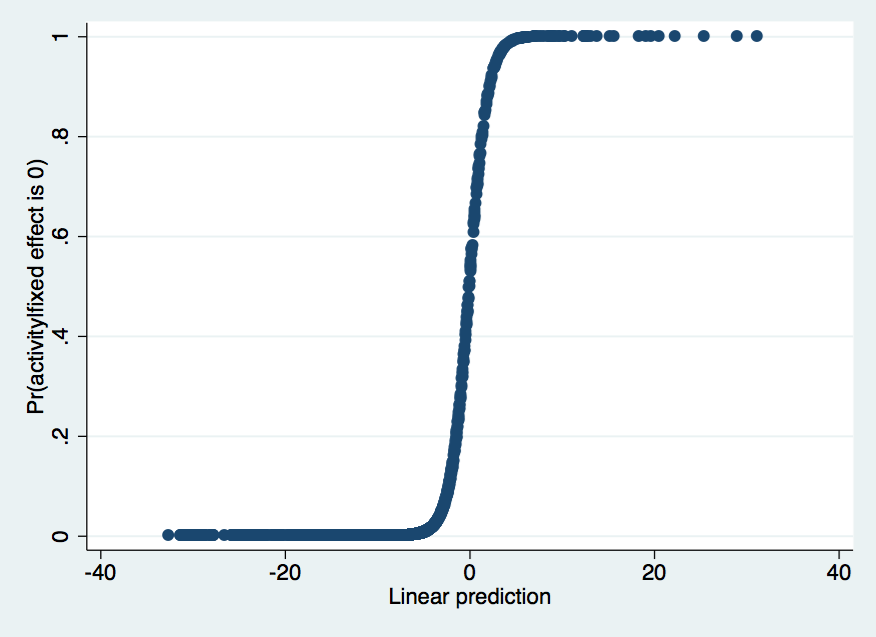
\includegraphics[width=.8 \textwidth]{PrAct_linPred}
	\caption{Predicted probability of Edgeryders users to become active as the linear prediction $x\beta$ based on number of comments received by community managers and other users increases.}
\label{fig:probActivityLinPredict}
\end{figure}

Table \ref{table:dydx} shows a point estimate the marginal effect of comments from the two sources (online community managers vs. other users) on the probability that a user will become active. Neither is significant. This turns out to be an artefact of the computation: the size of the marginal effect is computed fixing the value of regressors at their mean. The means of the variables in question are low. In the average period, the average Edgeryders user received 0.08 comments from online community managers and 0.09 comments from other users. This is consistent with what we know about patterns of human communication, which is sparse and bursty (\cite{holme2012temporal}). 

{
\def\onepc{$^{\ast\ast}$} \def\fivepc{$^{\ast}$}
\def\tenpc{$^{\dag}$}
\begin{table}[htbp]\centering
 \begin{tabular}{l c c c}\hline\hline 
\multicolumn{1}{c}
{\textbf{Variable}} & {\textbf{$dy/dx$}}  & \textbf{$Std. Err.$} & \textbf{$P > \lvert z \rvert$} \\ \hline
n. comments from community managers  &  .0000959  & .0004127 & 0.816 \\
n.  comments from other users  &  .0000165  & .000071 & 0.816\\
\hline
\end{tabular}
\caption{Marginal effects of the number of comments received by a user (both from community managers and from other users) on the probability of that user to become active. The estimates are computed under the assumption that regressors be fixed at their means. 
\label{table:dydx}}
\end{table}
}
A more intuitive approach is to estimate the elasticities of the probability of becoming active with respect to the number of comments received from each source. These are shown in table \ref{tab:elasticities}. They are both highly significant. In absolute terms, they are both small, but quite different. Receiving an extra comment by a community manager increases the probability that a user will become active by 10\%; but receiving one from another user will increase it by less than 2\%.

{
\def\onepc{$^{\ast\ast}$} \def\fivepc{$^{\ast}$}
\def\tenpc{$^{\dag}$}
\def\legend{\multicolumn{4}{l}{\footnotesize{Significance levels
:\hspace{1em} $\dag$ : 10\% \hspace{1em}
$\ast$ : 5\% \hspace{1em} $\ast\ast$ : 1\% \normalsize}}}
\begin{table}[htbp]\centering
 \begin{tabular}{l c c c}\hline\hline 
\multicolumn{1}{c}
{\textbf{Variable}} & {\textbf{$ey/ex$}}  & \textbf{$Std. Err.$} & \textbf{$P > \lvert z \rvert$} \\ \hline
n. comments from community managers  &  .1024245\onepc  & .0043113 & 0.000 \\
n. comments from other users  &  .01882\onepc  & .0032799 & 0.000\\
\hline
\end{tabular}
\caption{Elasticities of the probability that a user becomes active with respect to the number of comments received from community managers and from other users. The estimates are computed under the assumption that regressors be fixed at their means.
\label{tab:elasticities}}
\end{table}
}

Significant elasticities do not, per se, guarantee that the action of community managers will produce a large marginal effect in the online communities, unless the extra action (the differential increase in the regressor) is applied in a region of the distribution where the probability of the user being active is already reasonably high. We therefore turn to computing the marginal effect of the number of comments received from moderators on the probability that a user becomes active. Before we can proceed, however, we need an adjustment. In the model estimated so far, the mean of the predicted probability of a positive outcome (defined as the user
being active in the period) does not coincide with the proportion of users actually active across the dataset (table \ref{tab:flaw}). 

\begin{table}[htbp]\centering
 \begin{tabular}{l c c c}\hline\hline 
\multicolumn{1}{c}
{\textbf{Variable}} & {\textbf{Obs}}  & {\textbf{Mean}} & {\textbf{Std. Dev.}} \\ \hline
$prob$  &    84262   & .0023325  &  .0410453 \\
$active$  &  84262 &   .0181577  &  .1335221 \\
\hline
\end{tabular}\caption{Descriptive statistics for the probability of users to become active as predicted by the model ($prob$) and users actually being active ($active$).
\label{tab:flaw}}
\end{table}

This is caused by fact that the mean of the fixed effects $c_i$ is nonzero. To correct this, we need to add to the model a constant $\alpha$ such that: 

\begin{equation}
	 \frac{e^{mean(X_{i,t}\beta) + \alpha}}{1 + e^{mean(X_{i,t}\beta) + \alpha}} = \frac{\sum_{i = 1}^N \sum_{t = 1}^T active_{i,t}}{NT}
	 \label{eq:equationAlpha}
\end{equation}

In equation \ref{eq:equationAlpha}, $active_{i,t}$ takes value 1 if user $i$ is active at period $t$, and 0 otherwise; the $x_{i,t}\beta$ are the ones already estimated. The corrected model's linear predictions are unbiased, allowing us to compute marginal effects correctly. The right-hand side of equation \ref{eq:equationAlpha} is identical to the mean of the variable $active$ in table \ref{tab:flaw}. Replacing the appropriate values from table \ref{tab:flaw} yields:

\begin{equation}
	\frac{e^{-9.52 + \alpha}}{1 + e^{-9.52 + \alpha}} = 0.18
\end{equation}

\begin{equation}
	\alpha \simeq 8
	\label{eq:valueAlpha}
\end{equation}

We can now replace equation \ref{eq:valueAlpha} in to equation \ref{eq:equationAlpha} and proceed to estimate its marginal effects. Start by noting that, differentiating the right-hand side of \ref{eq:equationAlpha} with respect to $X$ yields:

\begin{equation}
	\frac{\partial Pr(A=1|X)}{\partial X} = \beta \frac{e^{X \beta + \alpha}}{(1 + e^{X \beta + \alpha})^2} 
\end{equation}

Replace the point estimates for $\beta_{cmrec}$, $\beta_{urec}$ and $\alpha$ to yield marginal effects of receiving one additional comments from, respectively, community managers and other users on the probability of being active in the period: 

\begin{equation}
	\frac{\partial Pr(A=1|X)}{\partial x_{cmrec}} = \beta_{cmrec} \frac{e^{ \beta_{cmrec} + \alpha}}{(1 + e^{x_{cmrec} \beta_{cmrec} + \alpha})^2} 
	\label{eq:marginal_x_cmrec}
\end{equation}

\begin{equation}
	\frac{\partial Pr(A=1|X)}{\partial x_{urec}} = \beta_{urec} \frac{e^{ \beta_{urec} + \alpha}}{(1 + e^{x_{urec} \beta_{urec} + \alpha})^2} 
	\label{eq:marginal_x_urec}
\end{equation}

Equations \ref{eq:marginal_x_cmrec} and \ref{eq:marginal_x_urec} allow us to "drill down" into the information contained in Table \ref{table:dydx} and study the marginal effects of receiving one additional comment after the same user has already received zero, one or more comments. To do so, we compute, for each observation and for both $x_{cmrec}$ and $x_{urec}$, the estimate of the marginal effect on the probability of the user being active. These are obtained plugging the observed regressor values, the computed value of $\alpha$ and the point estimates of the coefficient values into, respectively, equations \ref{eq:marginal_x_cmrec} and \ref{eq:marginal_x_urec}. We then repeat the procedure to compute the marginal effect of receiving comments from fellow participants in the Edgeryders community who are not online community managers. 

Plotting the frequency density of the two marginal effects shows that the comments of community managers have a greater activating marginal effect than those of non-community managers (Figure \ref{fig:marginalFxHisto}).

\begin{figure}
	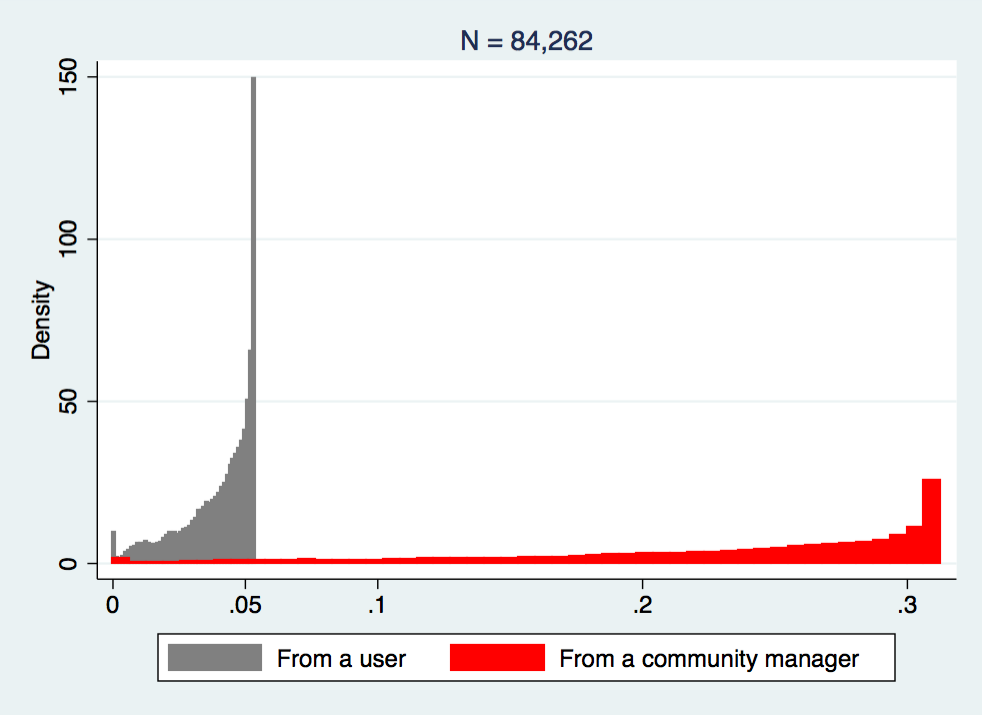
\includegraphics[width=.8 \textwidth]{Marginal_fx_histo}
	\caption{Frequency density of the marginal effect on the probability of being active of receiving a comment from online community managers and from other users in Edgeryders. Computed using point estimates for coefficient and observed values of regressors.}
\label{fig:marginalFxHisto}
\end{figure}

Marginal effects of regressors depend obviously on the values of regressors themselves. Receiving comments has generally decreasing returns on the probability of users becoming active. Fixing the value of all other regressors at their respective means and computing the marginal effects of both $x_{cmrec}$ and $x_{urec}$ as the number of comments received by users increase, we obtain the graph of Figure \ref{fig:marginalFxScat}. The marginal effect of $x{cmrec}$ is initially high (close to 0.3), but then decreases monotonically and quickly. That of $x{urec}$ starts at a much lower level (about 0.05), rises slightly to reach a maximum for $x{urec} = 2$, and then it decreases much more slowly.

\begin{figure}
	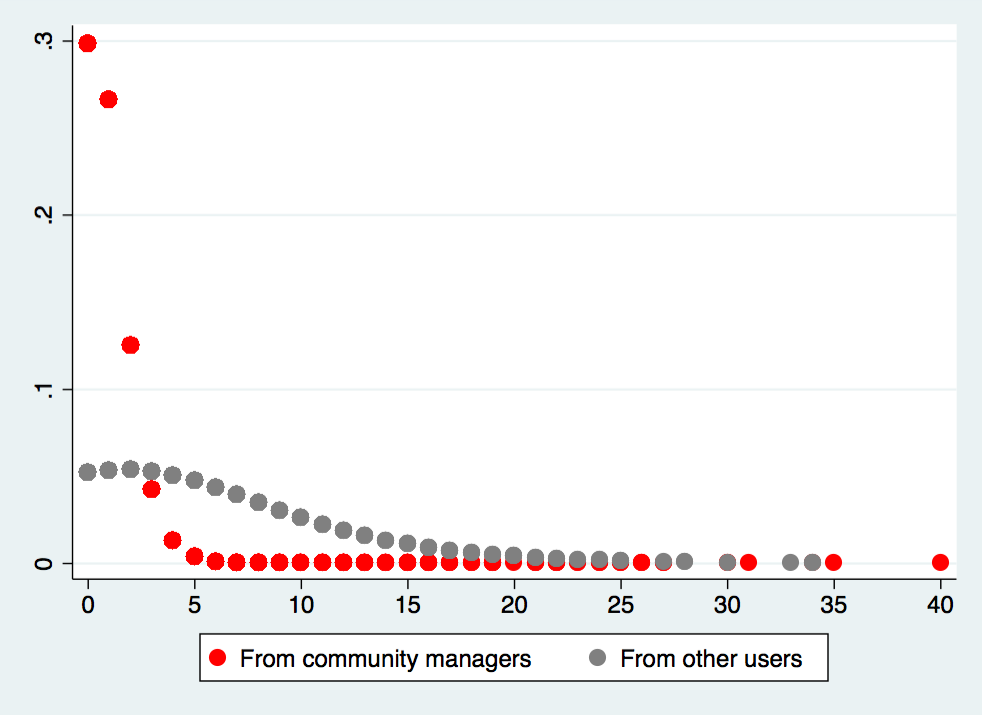
\includegraphics[width=.8 \textwidth]{Marginal_fx_scat}
	\caption{Marginal effect on the probability of being active of receiving a comment from online community managers and from other users in Edgeryders. Computed using point estimates for coefficient and mean values of regressors.}
\label{fig:marginalFxScat}
\end{figure}

This finding, illustrated by Figure \ref{fig:marginalFxScat} and Table \ref{tab:marginalProbabilityXcmrecObserved}, indicates support for Hypothesis \ref{hypothesis:policyWorksWell}, but only for low levels of $x_{cmrec}$.

Let's take a closer look, starting with the marginal effect of online community managers first. Tabulating the results according to the number of of comments received in each period by users, we derive Table \ref{tab:marginalProbabilityXcmrecObserved}. For users that have received no comments, the mass of the observations obtains for marginal probability values in or close to the 0.2-0.3 range. As the number of comments increases, predicted marginal probabilities decrease and quickly become indistinguishable from zero.

\begin{table}[htbp]\centering
	\begin{tabular}{c c | c  c  c  c | c}
 		& & \multicolumn{5}{c}{Marginal probability of user being active} \\
		& & \multicolumn{5}{c}{$X$ is at the observed value for each observation} \\
		\hline
		N. comments& & 0 - 0.1&0.1 - 0.2&0.2 - 0.3&over 0.3&Total \\
		\hline
		& mean & .06 & .15 & .26 & .31 & .23 \\ 
		0 & SE & .02 & .03 & .03 & .00 & .07 \\
		& N & 5,748&15,303&41,028&19,566&81,645 \\
		\hline
		 & mean & .04 & .14 & .25 & .31 & .15 \\
		1 & SE & .03 & .03 & .03 & .00 & .10 \\
		&N&438&308&362&111&1,219 \\
		\hline
		& mean & .03 & .14 & .25 & .31 & .07 \\
		2 & SE & .03 & . 03 & .03 & .00 & .08 \\
		& N&340&91&32&6&469 \\
		\hline
		& mean & .02 & .14 & . 25 & .31 & .04 \\
		3 & SE & .02 & .03 & .00 & .07 \\
		&N&223&8&13&2&246 \\
		\hline
		& mean & .01 & .12 & .25 & .31 & .04 \\
		4 & SE & .02 & .01 & .03 & .00 & .07 \\
		& N & 135 & 4 & 5 & 2 & 146 \\
		\hline
		& mean & .01 & .15 & .25 & .31 & .03 \\
		5 to 10 & SE & .02 & .03 &.03 & .00 & .08 \\
		& N&329&13&22&8&372 \\
		\hline
		& prob & .00 & .16 & .26 & .30 & .02 \\
		11 and above & SE & .01 & .03 & .04 & 0 & .05 \\
		& N &154&6&4&1&165 \\
		\hline
		& mean & .05 & .16 & .26 & .31 &.23 \\
		\textbf{Total} & SE & .03 & .03 & .03 & .00 & .08\\
		& N &7,367&15,733&41,466&19,696&84,262 \\
		\hline
	\end{tabular}
	\caption{Distribution of the observations according to the marginal effect of the user being active in the period with respect to receiving an extra comment from a community manager, and to the number of comments received in the same period. All other regressors enter the prediction function at the value observed for each observation.}

	\label{tab:marginalProbabilityXcmrecObserved}
\end{table}

Table \ref{tab:marginalProbabilityXcmrecObserved} has an interesting implication. The first and second comments any user receives are those with the highest (over .2) marginal effect on her activation in each period. Yet, community managers in Edgeryders write more than two comments to the same user in a relatively high number of instances. Of the 84,262 observations in our dataset, 2,617 are those for which the user received at least one comment from online community managers. Over a third (929) saw the user receiving three or more comments, having no predicted marginal effect on user activity in the period. We interpret these extra comments as exchanges, with community managers and users commenting (presumably) the same content within the same time period. This is not necessarily ineffective behaviour: online community managers might be driven by purposes other than activation, for example helping to give users a good experience of the community.  

We now turn to the marginal effect on the probability of being active of comments written by users who are not online community managers. Table \ref{tab:marginalProbabilityXurecObserved} is less informative than Table \ref{tab:marginalProbabilityXcmrecObserved}, given that the predicted marginal effect of $x_{urec}$ is smaller and more clustered around a single value than that of $x_{cmrec}$. Still, we do observe that the predicted marginal effect of the former is greater than .05 about one third of the times when $x_{urec} = 0$. As $x_{urec}$ increases, this proportion decreases, as does the average marginal effect.

\begin{table}[htbp]\centering
	\begin{tabular}{c c | c  c | c}
 		& & \multicolumn{3}{c}{Marginal probability of user being active} \\
		& & \multicolumn{3}{c}{$X$ is at the observed value for each observation} \\
		\hline
		N. comments& & 0 - 0.05&0.05 - 0.1&Total \\
		\hline
		& mean & .03 & .05 & .04 \\ 
		0 & SE & .01 & .00 & .01 \\
		& N & 56,183&25,716&81,899 \\
		\hline
		 & mean & .02 & .05 & .03 \\
		1 & SE & .02 & .00 & .02 \\
		&N&871 & 192 & 1,063 \\
		\hline
		& mean & .02 & .08 & .02 \\
		2 & SE & .02 & .00 &.02 \\
		& N& 425 & 47 & 472 \\
		\hline
		& mean & .01 & .05 & .01 \\
		3 & SE & .01 & .00 & .02 \\
		&N& 235 & 13 & 248\\
		\hline
		& mean & .01 & .05 & .01 \\
		4 & SE & .01 & .00 & .02 \\
		& N & 136 & 8 & 144 \\
		\hline
		& mean & .01 & .05 & .01  \\
		5 to 10 & SE & .01 & .00 & .01 \\
		& N&309&14& 323 \\
		\hline
		& prob & . & .00 \\
		11 and above & SE & .01 & . & .01\\
		& N &113 & 0 & 113\\
		\hline
		& mean & .03 & .05 & .04 \\
		\textbf{Total} & SE & .01 & .00 & .01\\
		& N & 58,272 & 25,990 & 84262 \\
		\hline
	\end{tabular}
	\caption{Distribution of the observations according to the marginal effect of the user being active in the period with respect to receiving an extra comment from a non-community manager, and to the number of comments received in the same period. All other regressors enter the prediction function at the value observed for each observation.}
	\label{tab:marginalProbabilityXurecObserved}
\end{table}

